\subsection{Entwurfsalternativen}
Neben dem in Abbildung \ref{fig:Bild1} gezeigten Entwurf gibt es drei andere Alternativen. Die ersten beiden Entwurfsalternativen beziehen sich dabei nur auf die Aufteilung, welche Komponenten in welcher Programmiersprache programmiert werden. Die dritte Alternative bezieht sich dabei auf die Datenbank.
\subsubsection{1. Entwurfsalternative}

\begin{figure}[h]
  \centering
     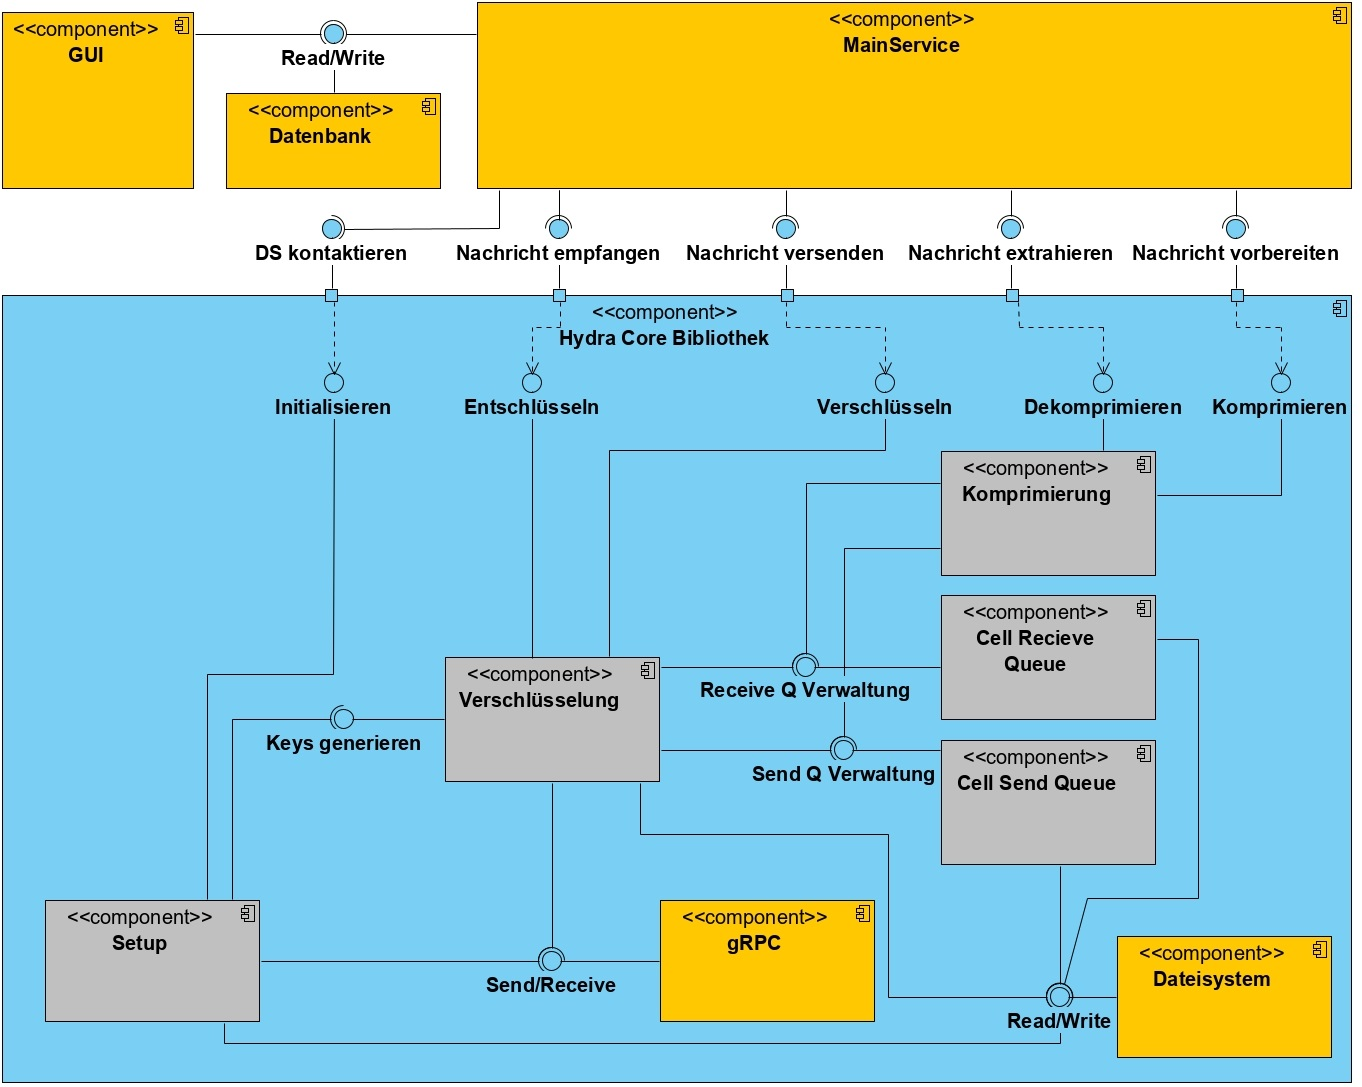
\includegraphics[width=0.9\textwidth]{diagramme/Component_Diagram_E1.jpg}
  \caption{1. Entwurfsalternative}
  \label{fig:Bild2}
\end{figure}

In der ersten Entwurfsalternative ist im Unterschied zu dem in Abbildung \ref{fig:Bild1} gezeigten Entwurf sowohl die Netzwerkschnittelle \ac{gRPC} als auch das Dateisystem  in Kotlin programmiert. Das Ganze hat aber entscheidende  Nachteile:
\begin{itemize}
\item[1)] Das Hydra-System schreibt uns \ac{gRPC} als Netzwerkschnittstelle vor und liefert uns bereits ein Protocol Buffer, welcher in C++ programmiert ist. Es wäre also unnötig, diese Komponente nochmals neu in Kotlin zu programmieren.
\item[2)]Das Dateisystem verwaltet in der \ac{HCB} ausschließlich Dateien, auf die Komponenten zugreifen, welche in C++ programmiert sind. Somit wäre es inkonsistent und unnötig kompliziert, das Dateisystem in Kotlin zu programmieren
\end{itemize}

Aus den genannten Gründen ist diese Entwurfsalternative ungeeignet.

\subsubsection{2. Entwurfsalternative}

\begin{figure}[h]
  \centering
     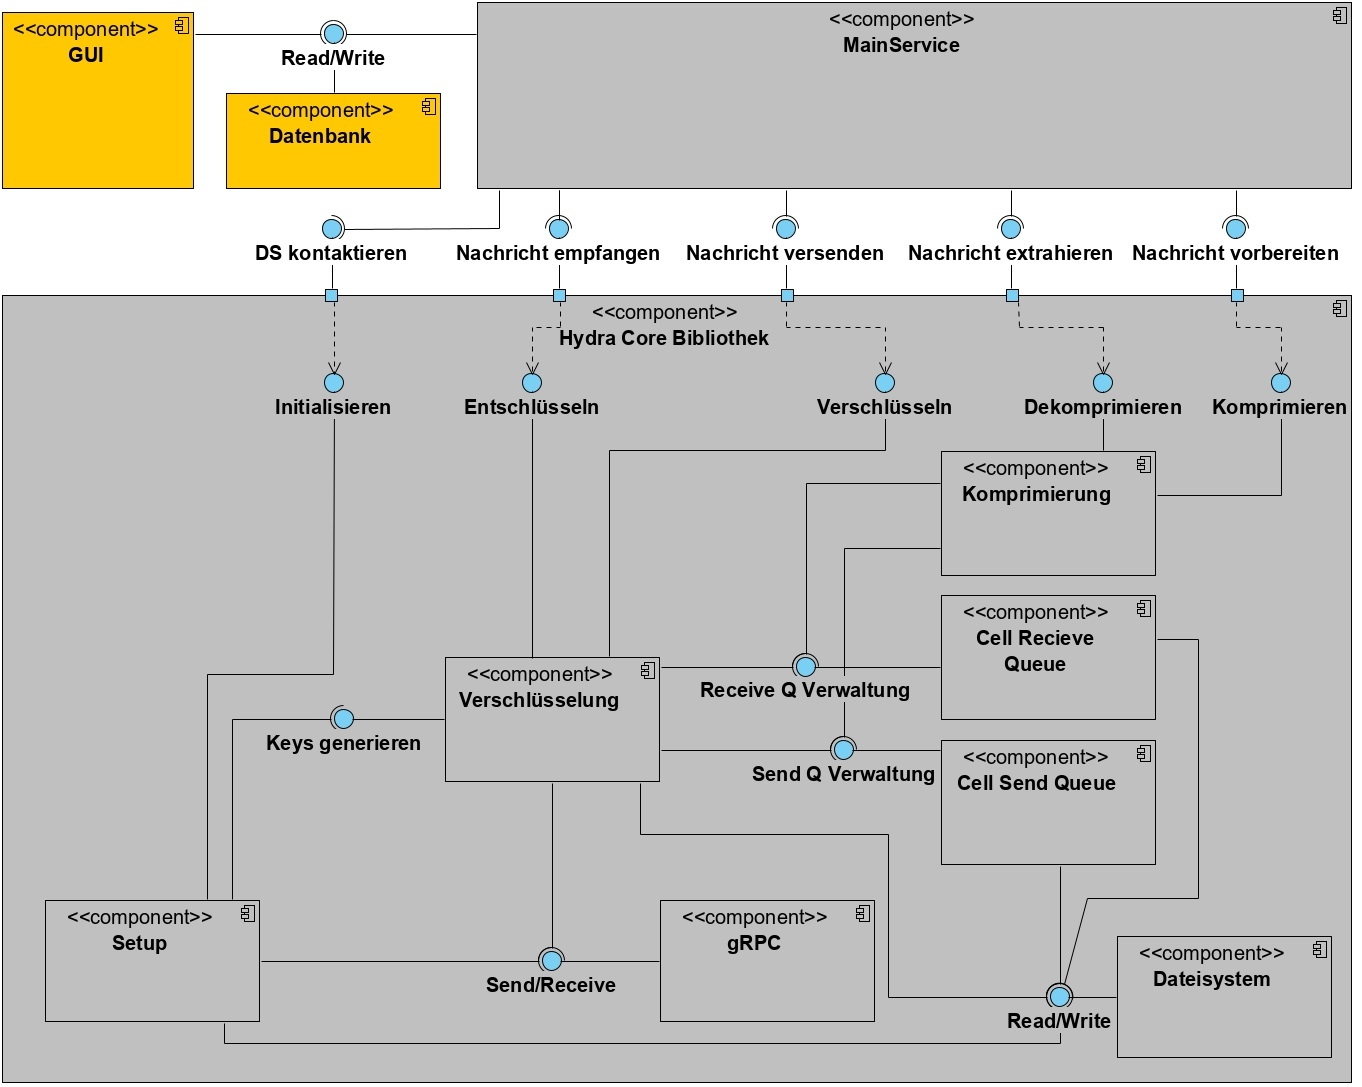
\includegraphics[width=0.9\textwidth]{diagramme/Component_Diagram_E3.jpg}
  \caption{2. Entwurfsalternative}
  \label{fig:Bild3}
\end{figure}

In der zweiten Entwurfsalternative ist neben der \ac{HCB} auch der \ac{MS} in C++ programmiert. Doch dies hat wieder einen entschiedenen Nachteil: Der \ac{MS} muss mit dem Android System kommunizieren. Da Kotlin extra für die Android-Entwicklung entwickelt worden ist, würde man das System nur unnötig schwer gestalten, wenn man den \ac{MS} in C++ programmiert. 

Aus diesem Grund ist auch diese Entwurfsalternative ungeeignet.
\newpage
\subsubsection{3. Entwurfsalternative}

\begin{figure}[h]
  \centering
     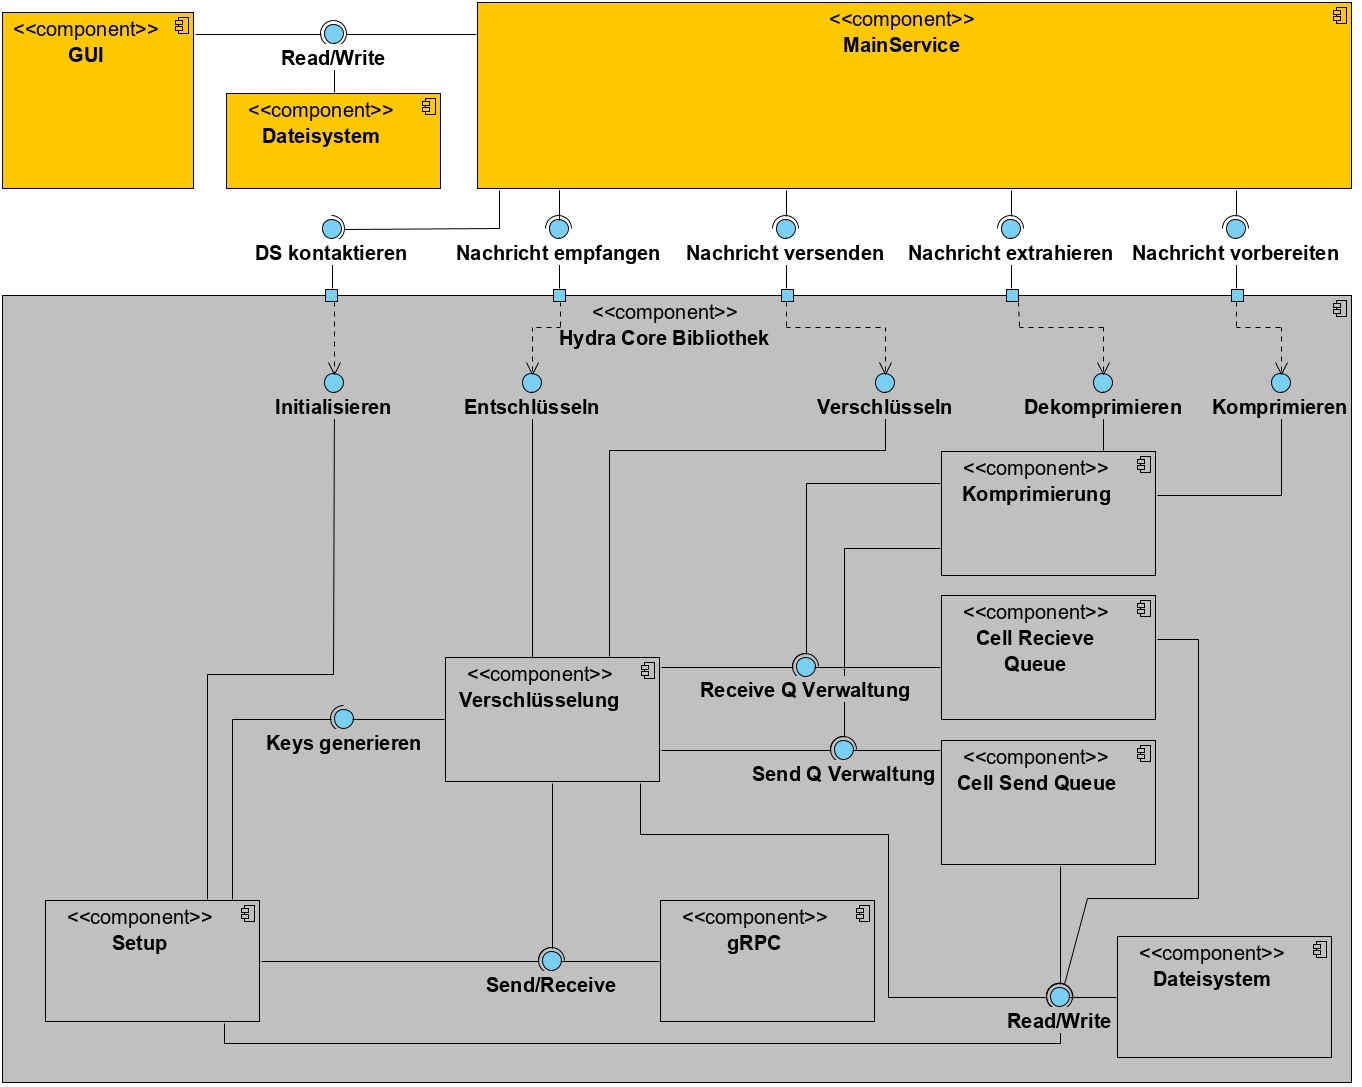
\includegraphics[width=0.9\textwidth]{diagramme/Component_Diagram_E4.jpg}
  \caption{3. Entwurfsalternative}
  \label{fig:Bild4}
\end{figure}

In der dritten Entwurfsalternative wird anstatt einer Datenbank ein einfaches Dateisystem genutzt. Aber auch diese Alternative hat mehrere Nachteile:
\begin{itemize}
\item[1)]Da sowohl der \ac{MS} also auch die \ac{GUI} auf den Chatverlauf bzw. das Kontaktbuch zugreifen, müsste ein wechselseitiger Ausschluss implementiert werden. 
\item[2)]Da die Kommunikation zwischen dem \ac{MS} und der \ac{GUI} über das Dateisystem läuft, müssen Such-Operationen ausgeführt werden (um neue Nachrichten zu entdecken usw.). Genau solche Operationen sind sehr effizient in Datenbanken implementiert und müssen hier selbst implementiert werden. 
\end{itemize}

Aus den genannten Gründen ist auch diese Entwurfsalternative eher ungeeignet.
